% schéma d'une échelle de qualité pour les méthodes par comparaison avec échelle d'évaluation continue

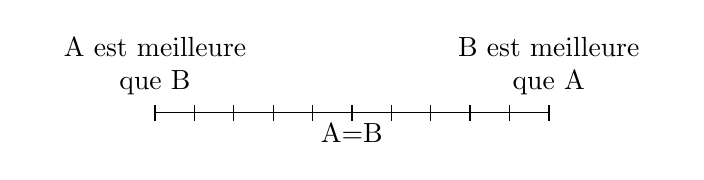
\begin{tikzpicture}
  \draw (0,0) -- (5,0);
  \draw[thick] (5,-0.1) -- (5,0.1)  node[above, text width=3cm, text centered] {B est meilleure que A};
  \draw (4.5,-0.1) -- (4.5,0.1);
  \draw (4,-0.1) -- (4,0.1);
  \draw (3.5,-0.1) -- (3.5,0.1);
  \draw (3,-0.1) -- (3,0.1);
  \draw[thick] (2.5,-0.1) -- (2.5,0.1) node [below=0.1cm] {A=B};
  \draw (2,-0.1) -- (2,0.1);
  \draw (1.5,-0.1) -- (1.5,0.1);
  \draw (1,-0.1) -- (1,0.1);
  \draw (0.5,-0.1) -- (0.5,0.1);
  \draw[thick] (0,-0.1) -- (0,0.1) node[above, text width=3cm, text centered] {A est meilleure que B};
\end{tikzpicture}